\chapter{Results}


\section{Model Evaluation}


\subsection{Comparison of Results in NSTL with COLMAP and OpenCV}

To validate the 3D Gaussian Splatting method in the Neural Space Time Lab (NSTL), a new dataset was captured and prepared using two different calibration approaches: COLMAP and OpenCV. 
The scene was trained, rendered, and evaluated using SSIM, PSNR, and LPIPS metrics to assess the impact of the calibration method on reconstruction quality, as described in the methodology section (Chapter~\ref{chap:Methodik}).

The results are summarized in Table~\ref{tab:3dgs_results_nstl}. 
Both calibration methods achieve high reconstruction quality, with COLMAP showing slightly better metric values. 
The differences can be attributed to the optimized estimation of camera poses through the structure-from-motion (SfM) procedure.

\begin{table}[h]
\centering
\caption{Comparison of metrics for the scene from the NSTL dataset.}
\label{tab:3dgs_results_nstl}
\begin{tabular}{lccc}
\toprule
& SSIM $\uparrow$ & PSNR (dB) $\uparrow$ & LPIPS $\downarrow$\\
\midrule
COLMAP & 0.931 & 35.58 & 0.18 \\
OpenCV & 0.927 & 34.56 & 0.252\\
\bottomrule
\end{tabular}
\end{table}

Figure~\ref{fig:3dgs_COLMAP} shows a visual comparison for the COLMAP-based reconstruction. 
The rendered image closely resembles the ground truth, with clear textures and edges in the central region, while slight blurring is visible near the floor and image borders.

Figure~\ref{fig:3dgs_opencv} presents the OpenCV-based reconstruction. 
Texture fidelity in the central region remains high, but quality decreases more noticeably toward the edges, particularly at the floor and in background elements such as a ladder.

\begin{figure}[h]
    \centering
    \subfloat[Ground Truth]{%
        \includegraphics[width=0.48\linewidth]{bilder/Results/3dgs/3dgs_COLMAP_gt.jpg}%
    }
    \hfill
    \subfloat[Rendered Image]{%
        \includegraphics[width=0.48\linewidth]{bilder/Results/3dgs/3dgs_COLMAP_render.jpg}%
    }
    \caption{Comparison between ground truth and rendered image using COLMAP camera poses: The reconstruction shows clear textures in the central region, with minor blurring near the floor and image borders.}
    \label{fig:3dgs_COLMAP}
\end{figure}

\begin{figure}[h]
    \centering
    \subfloat[Ground Truth]{%
        \includegraphics[width=0.48\linewidth]{bilder/Results/3dgs/3dgs_OpenCV_gt.png}%
    }
    \hfill
    \subfloat[Rendered Image]{%
        \includegraphics[width=0.48\linewidth]{bilder/Results/3dgs/3dgs_OpenCV_render.png}%
    }
    \caption{Comparison between ground truth and rendered image using OpenCV calibration: The reconstruction maintains good texture fidelity in the central region, with stronger blurring near the floor and background.}
    \label{fig:3dgs_opencv}
\end{figure}

Despite the slightly better metrics of COLMAP, OpenCV is preferred for NSTL applications, as explained in the methodology section (Chapter~\ref{chap:Methodik}). 
Deterministic calibration with OpenCV provides a coordinate system in real-world units, ensuring precise and reproducible spatial positioning. 
This is crucial for integration with other NSTL systems and for future extensions to dynamic scenes using 4D Gaussian Splatting. 
The similar reconstruction quality in the central region demonstrates that OpenCV, despite slightly lower metrics, is a robust alternative due to its consistency and lower dependence on scene-specific optimizations. 
These results provide a solid foundation for the investigation of dynamic scenes in the following sections.




\section{Composition Pipeline Evaluation}

This chapter presents a qualitative evaluation of the proposed multi-camera compositing and dynamic scene generation pipeline. 
In the absence of complete ground-truth annotations, the analysis focuses on visual consistency, temporal coherence, and scene-level generalization across multiple reconstruction and rendering configurations. 
All results were produced using the same calibrated multi-camera rig under identical rendering parameters, without manual post-processing unless explicitly stated.

\section{Compositional Scene Generation}
Figure~\ref{fig:composition} illustrates how the proposed compositing pipeline integrates multiple independently reconstructed Gaussian Splatting models into a single, globally aligned scene. 
Each row in the figure shows one configuration step, starting from a single-object placement and progressing toward increasingly populated scenes that combine both static and dynamic objects.
For each configuration, the corresponding RGB renderings, depth maps, bounding boxes, and segmentation overlays are presented to demonstrate multi-modal coherence.

A central advantage of the system is that all semantic annotations, including instance masks, class indices, and bounding boxes, are generated automatically and remain geometrically consistent across all rendered views. 
Since every 3D model is represented as Gaussian primitives within a shared coordinate system, mask generation requires no additional training or inference using segmentation networks. 
All semantic labels are deterministically derived from the compositing process itself, ensuring reproducible and noise-free annotations.

The modular design of the pipeline further enables high scene variability. 
Objects can be translated, rotated, scaled, or duplicated directly in 3D space without retraining or manual re-annotation. 
This flexibility allows large-scale dataset creation with controlled variation in object arrangement and spatial relationships. 
In practice, the same set of Gaussian models can be reused across numerous novel compositions while preserving consistent geometry, color, and semantic labeling, making the approach well suited for scalable and reproducible synthetic dataset generation.

\begin{figure*}[t]
    \centering
    \includegraphics[width=\textwidth]{Grafiken/Composition.pdf}
    \caption{
        \textbf{Compositional scene generation.}
        Example of multi-object scenes composed from independently reconstructed Gaussian Splatting models. 
        Each row shows one scene configuration with RGB, depth, bounding boxes, and segmentation overlays.
        All semantic annotations are generated automatically and remain spatially consistent across views.
    }
    \label{fig:composition}
\end{figure*}

\section{Multi-view Occlusion Handling}
To assess the robustness of the compositing mechanism under occlusions, 
Figure~\ref{fig:occlusion} shows segmentation overlays from two viewpoints of a scene containing interacting dynamic subjects. 
Even when large parts of one subject are occluded, the instance masks remain spatially consistent and tightly aligned with visible contours. 
This demonstrates that the rendering process preserves correct inter-object depth ordering and instance integrity across multiple perspectives. 
Such behavior is crucial for generating reliable training data for tasks such as instance segmentation or 3D scene understanding, where stable occlusion boundaries are essential.

\begin{figure}[ht]
    \centering
    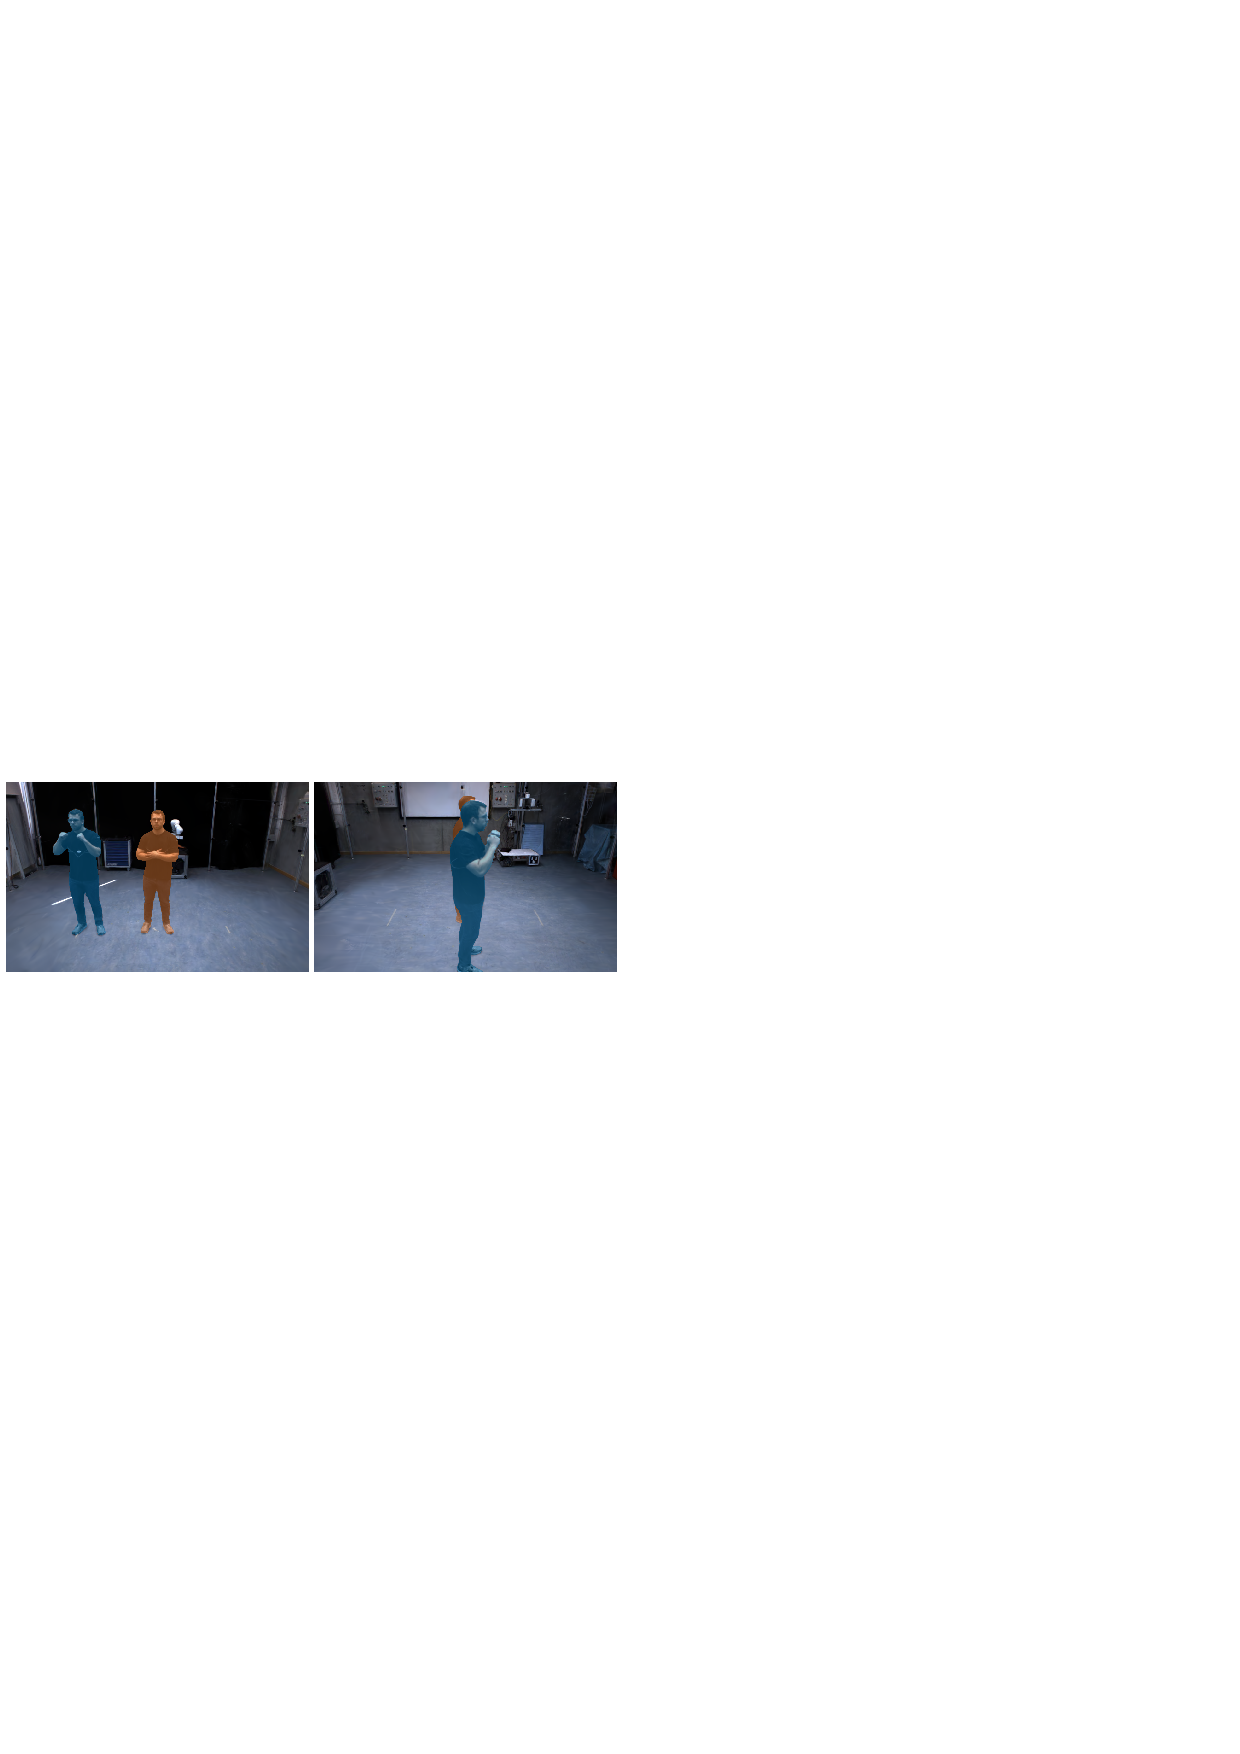
\includegraphics[width=\linewidth]{Grafiken/Oclusion.pdf}
    \caption{
        \textbf{Occlusion handling across views.}
        Segmentation overlays from front and side viewpoints of two interacting subjects.
        Even under strong mutual occlusion, instance masks remain consistent and well aligned with visible contours.
    }
    \label{fig:occlusion}
\end{figure}

\section{Scene Generalization}
Figure~\ref{fig:generalization} demonstrates the adaptability of the proposed system by recontextualizing dynamic subjects within a novel virtual environment reconstructed from real imagery using COLMAP \cite{schoenberger2016sfm}. 
The reconstructed environment provides realistic geometry and camera poses that serve as a spatial reference for compositing. 
Dynamic subjects are seamlessly integrated into the new setting, maintaining correct spatial alignment, depth consistency, and segmentation coherence. 
By decoupling object-level Gaussian models from a specific environment, the system enables arbitrary recombination of dynamic and static assets across scenes without retraining. 
This generalization capability supports large-scale variation in scene composition and facilitates applications such as domain adaptation, robustness evaluation, and synthetic-to-real transfer.

\begin{figure}[ht]
    \centering
    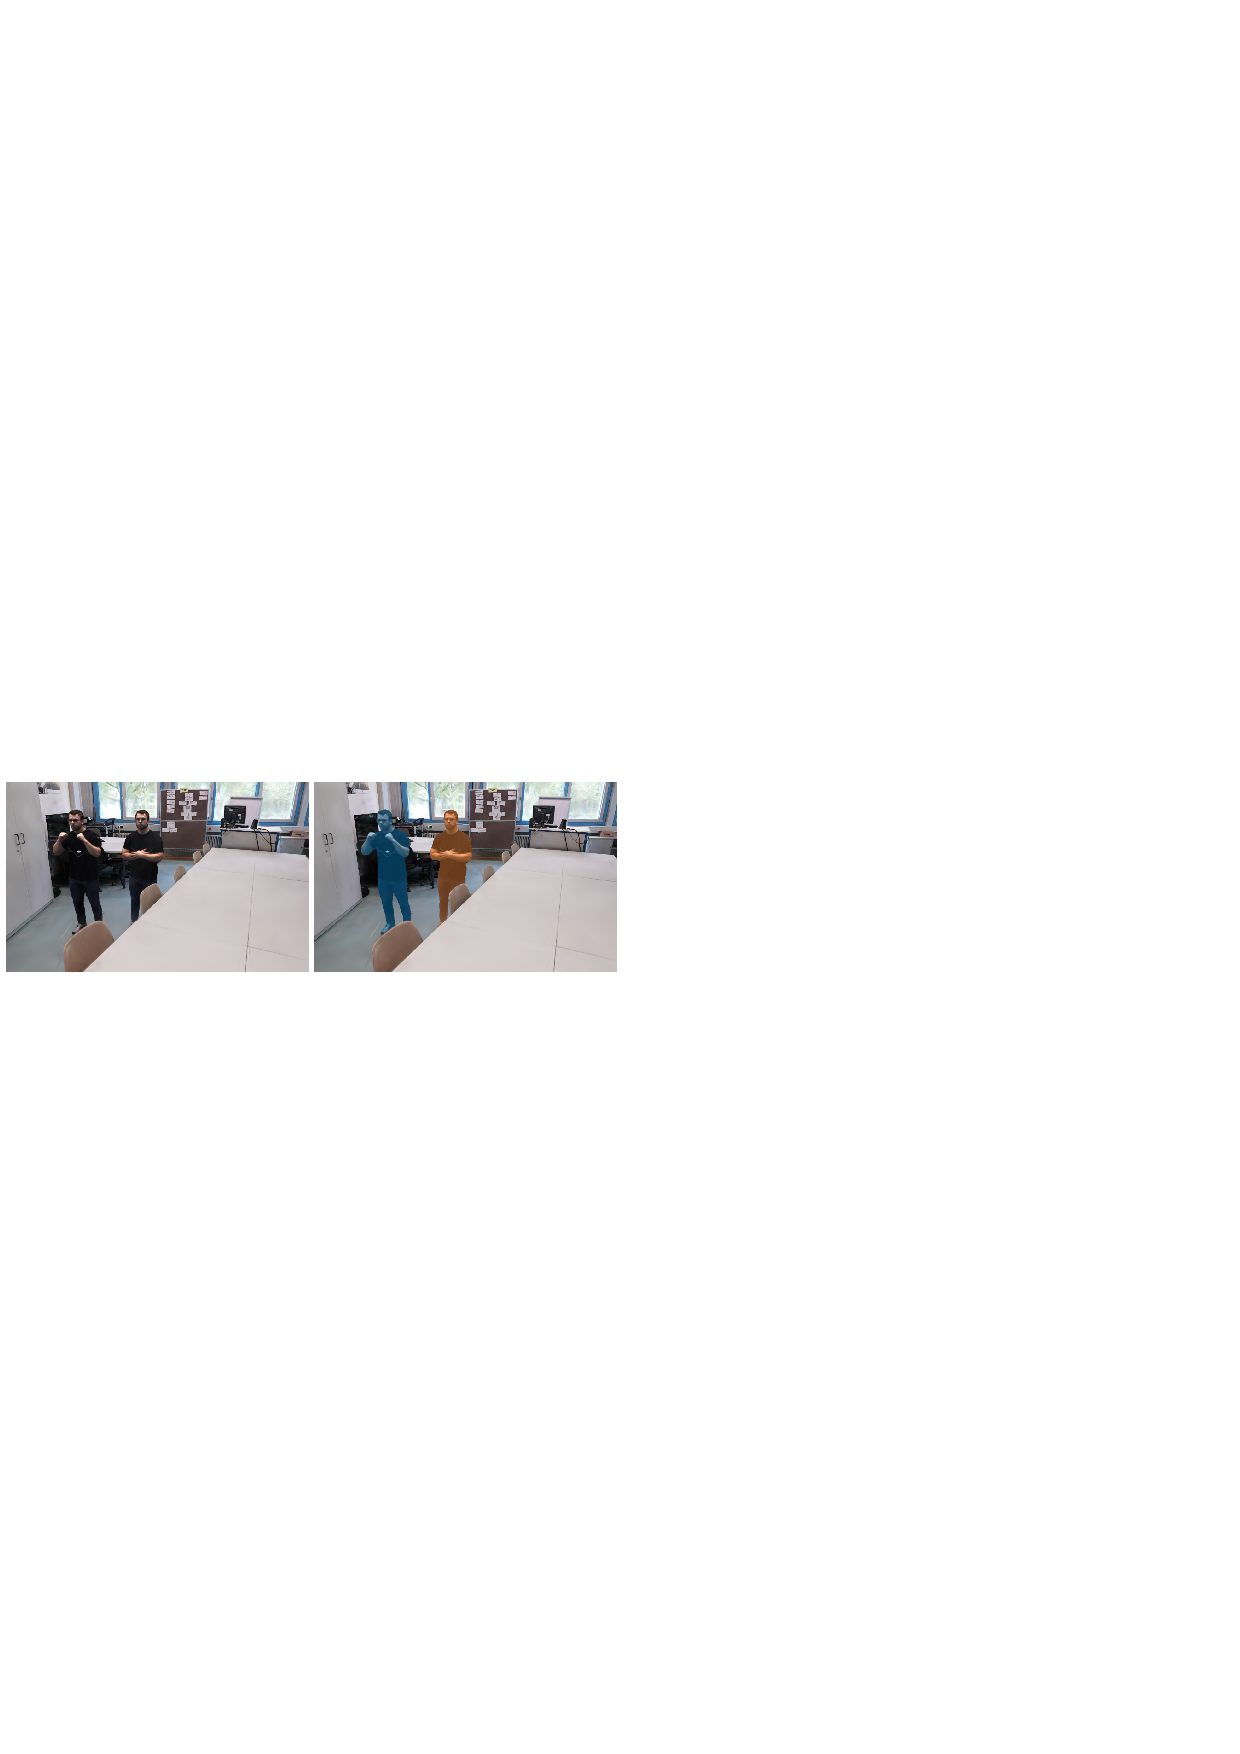
\includegraphics[width=\linewidth]{Grafiken/room_transfer.pdf}
    \caption{
        \textbf{Scene generalization and recontextualization.}
        Dynamic subjects composited into a novel virtual environment reconstructed with COLMAP.
        The system maintains consistent geometry and segmentation alignment across domains, 
        demonstrating flexible recontextualization of pre-trained Gaussian models.
    }
    \label{fig:generalization}
\end{figure}

\section{Temporal Consistency in Dynamic Scenes}
Dynamic scene rendering enables the generation of temporally coherent 4D datasets suitable for applications such as activity recognition, pose estimation, or motion segmentation. 
Figure~\ref{fig:temporal} shows representative frames from a dynamic sequence of a moving subject. 
The RGB and segmentation overlays reveal smooth and consistent motion over time, with stable geometry and accurate alignment across frames. 
Each time step preserves object structure and surface continuity, indicating that the Gaussian-based transformation updates produce interpretable and stable temporal behavior. 
This capability allows scalable synthesis of realistic dynamic sequences without requiring explicit motion capture or manual supervision.

\begin{figure*}[t]
    \centering
    \includegraphics[width=\textwidth]{Grafiken/time.pdf}
    \caption{
        \textbf{Dynamic scene generation.}
        Representative time steps of a moving subject with RGB and segmentation overlays.
        The consistent motion and geometry across frames demonstrate temporally stable 4D rendering.
    }
    \label{fig:temporal}
\end{figure*}

\section{Qualitative Pose Estimation}
Figure~\ref{fig:keypoints} (top row) shows qualitative 6D pose estimates for a dynamic human sequence across four time steps. 
Each frame visualizes the canonical object coordinate system derived from the aggregated Gaussian transformations. 
Although no ground-truth pose data are available, the estimated coordinate axes evolve consistently and reflect plausible orientation changes relative to the subject’s motion. 
This indicates that Gaussian-based transformation tracking provides a reliable approximation of object-level motion, suitable for downstream tasks such as pose refinement or motion analysis.

\section{Keypoint Propagation}
The lower row of Figure~\ref{fig:keypoints} visualizes the temporal keypoint propagation results obtained with a Detectron2-based detector \cite{Detectron22020}. 
Initial 2D keypoints are detected in a reference frame and projected into 3D by associating them with the nearest Gaussian centroids of the corresponding subject. 
As a result, keypoints are anchored on the object surface rather than the true anatomical joints, but they remain spatially coherent throughout the sequence. 
The keypoints are subsequently propagated in time according to the motion of the underlying Gaussians.

Temporal stability is observed across most body regions, particularly in the upper body where Gaussian density is high and motion is well captured. 
Minor deviations appear in areas with sparse or unstable Gaussian coverage, such as the knees or hips, leading to small temporal inconsistencies or spatial offsets. 
Despite these limitations, the propagation maintains overall semantic coherence and demonstrates that the Gaussian-based motion field can sustain meaningful correspondences over time. 
This behavior provides a promising foundation for future integration with articulated motion priors or learned joint-space constraints.

\begin{figure*}[t]
    \centering
    \includegraphics[width=\textwidth]{Grafiken/keypoints.pdf}
    \caption{
        \textbf{Qualitative analysis of pose and keypoint propagation.}
        Four frames of a dynamic subject showing estimated object poses (top) and propagated keypoints (bottom).
        The coordinate systems evolve consistently over time, while keypoint trajectories remain coherent despite local misalignments.
    }
    \label{fig:keypoints}
\end{figure*}

% \section{Summary}
% Overall, these qualitative results highlight that our framework can produce temporally stable geometric and semantic representations for dynamic scenes. 
% Although both pose and keypoint estimation currently rely on unsupervised tracking without ground-truth reference, the observed consistency across time demonstrates the potential of our 4D Gaussian representation as a foundation for future work in motion analysis, activity recognition, and articulated model learning.



